\documentclass{article} 

\usepackage{../style/nips13submit,times}
\usepackage{hyperref}
\usepackage{url}








\usepackage{latexsym}
\usepackage{amsmath}
\usepackage{multirow}
\usepackage{url}
\usepackage{algorithm}
\usepackage[noend]{algorithmic}
\usepackage{CJK}
\usepackage{subfigure}


\newif\ifcomment\commentfalse
% Preamble file contains handy macros and most packages you might want to use.
% At the start are packages that conflict with various styles.  Don't add them
% in!  Just put it in your main TeX file instead.

% Do not put either of these (subfigure or subfloat) into the preamble
% - they clash.  Use them in the final LaTeX document
% \usepackage{subfigure}
% \suepackage{subfloat}

% Do not use times in the preamble!  It just causes problems with some
% publication chairs (e.g., ICML 2013).  If you want it, put it in your own
% document.
% \usepackage{times}


% Breaks ACM-SIG style
% \usepackage{titlesec}
% \usepackage{amsthm}
% \usepackage{nomencl}

% comment out the following line, as it conflicts with aistats2012.sty
%\usepackage{caption}

% This is required by NSF.  Do not remove; if it conflicts with
% another package, fix that problem without removing this from
% Preamble.
% Unless for AAAI ... this needs a new bibfile that plays well with hyperref.
%\usepackage[a-1b]{pdfx}

% Below should be safe
\usepackage{framed}
\usepackage{mdwlist}
\usepackage{latexsym}
\usepackage{colortbl}
\usepackage{xcolor}
\usepackage{nicefrac}
\usepackage{booktabs}
\usepackage{amsfonts}
\usepackage[T1]{fontenc}
\usepackage{bold-extra}
\usepackage{amsmath}
\usepackage{amssymb}
\usepackage{bm}
\usepackage{graphicx}
\usepackage{mathtools}
\usepackage{microtype}
\usepackage{multirow}
\usepackage{multicol}
% Don't use hyperref or url, as it can screw up AAAI / ICML formatting
%\usepackage{url}
\usepackage{latexsym,comment}
\usepackage[normalem]{ulem}

\newcommand{\breakalign}{\right. \nonumber \\ & \left. \hspace{2cm}}



\newcommand{\feat}[1]{{\small \texttt{#1}}}
\newcommand{\act}[1]{{\small \texttt{#1}}}
\newcommand{\ngram}[0]{$n$-gram}
\newcommand{\topic}[1]{\underline{#1}}
\newcommand{\gem}[1]{\mbox{\textsc{gem}}}
\newcommand{\abr}[1]{\textsc{#1}}
\newcommand{\camelabr}[2]{{\small #1}{\textsc{#2}}}
\newcommand{\abrcamel}[2]{{\textsc #1}{\small{#2}}}
\newcommand{\grammar}[1]{{\color{red} #1}}
\newcommand{\explain}[2]{\underbrace{#2}_{\mbox{\footnotesize{#1}}}}
\newcommand{\dir}[1]{\mbox{Dir}(#1)}
\newcommand{\bet}[1]{\mbox{Beta}(#1)}
\newcommand{\py}[1]{\mbox{\textsc{py}}(#1)}
\newcommand{\td}[2]{\mbox{\textsc{TreeDist}}_{#1} \left( #2 \right)}
\newcommand{\yield}[1]{\mbox{\textsc{Yield}} \left( #1 \right)}
\newcommand{\mult}[1]{\mbox{Mult}( #1)}
\newcommand{\wn}{\textsc{WordNet}}
\newcommand{\twentynews}{\textsc{20news}}
\newcommand{\g}{\, | \,}
\newcommand{\Gam}[1]{\Gamma \left( \textstyle #1 \right)}
\newcommand{\LG}[1]{\log \Gamma \left( \textstyle #1 \right)}
\newcommand{\Pois}[1]{\mbox{Poisson}(#1)}
\newcommand{\pcfg}[3]{#1_{#2 \rightarrow #3}}
\newcommand{\grule}[2]{#1 \rightarrow #2}
\newcommand{\kl}[2]{D_{\mbox{\textsc{KL}}} \left( #1 \,||\, #2 \right)}

\newcommand{\digambig}[1]{\Psi \left( #1 \right) }
\newcommand{\digam}[1]{\Psi \left( \textstyle #1 \right) }
\newcommand{\ddigam}[1]{\Psi' \left( \textstyle #1 \right) }


\renewenvironment{quote}
               {\list{}{\rightmargin\leftmargin}%
                \item\relax\small\ignorespaces}
               {\unskip\unskip\endlist}

\DeclareMathOperator*{\argmax}{arg\,max}
\DeclareMathOperator*{\argmin}{arg\,min}
\newcommand{\bmat}[1]{\text{\textbf{#1}}}
\newcommand{\bvec}[1]{\boldsymbol{#1}}

%\newcommand{\email}[1]{ {\small \href{mailto://#1}{\texttt{#1} }  }}
\newcommand{\emaillink}[1]{ {\small \href{mailto://#1}{\texttt{#1}}}}
\newcommand{\smallemaillink}[2]{ {\small \href{mailto://#2}{\texttt{#1}}}}

% JBG: Consider renaming from \ch to \zh because of conflict when adding Cyrillic
\newcommand{\ch}[1]{\begin{CJK*}{UTF8}{gbsn}#1\end{CJK*}}

\newcommand{\e}[2]{\mathbb{E}_{#1}\left[ #2 \right] }
\newcommand{\h}[2]{\mathbb{H}_{#1}\left[ #2 \right] }
\newcommand{\ind}[1]{\mathds{1}\left[ #1 \right] }
\newcommand{\ex}[1]{\mbox{exp}\left\{ #1\right\} }
\newcommand{\D}[2]{\frac{\partial #1}{\partial #2}}
\newcommand{\elbo}{\mathcal{L}}

\newcommand{\hidetext}[1]{}
\newcommand{\ignore}[1]{}

\newcommand{\todo}[1]{\textcolor{red}{{\bf TODO: #1}}}

\ifcomment
\newcommand{\pinaforecomment}[3]{\colorbox{#1}{\parbox{.8\linewidth}{#2: #3}}}
\else
\newcommand{\pinaforecomment}[3]{}
\fi

\newcommand{\jbgcomment}[1]{\pinaforecomment{red}{JBG}{#1}}
\newcommand{\mjpcomment}[1]{\pinaforecomment{blue}{MJP}{#1}}
\newcommand{\czcomment}[1]{\pinaforecomment{orange}{chen}{#1}}
\newcommand{\ffcomment}[1]{\pinaforecomment{red}{FF}{#1}}
\newcommand{\fpcomment}[1]{\pinaforecomment{green}{FP}{#1}}
\newcommand{\yhcomment}[1]{\pinaforecomment{green}{YH}{#1}}
\newcommand{\hhecomment}[1]{\pinaforecomment{blue}{HH}{#1}}
\newcommand{\tncomment}[1]{\pinaforecomment{blue}{TN}{#1}}
\newcommand{\mnicomment}[1]{\pinaforecomment{green}{Mohit}{#1}}
\newcommand{\prcomment}[1]{\pinaforecomment{lightblue}{Pedro}{#1}}
\newcommand{\fscomment}[1]{\pinaforecomment{orange}{Shi}{#1}}
\newcommand{\vmcomment}[1]{\pinaforecomment{yellow}{Varun}{#1}}
\newcommand{\rscomment}[1]{\pinaforecomment{yellow}{Richard}{#1}}
\newcommand{\jszcomment}[1]{\pinaforecomment{green}{JSG}{#1}}
\newcommand{\ascomment}[1]{\pinaforecomment{blue}{AS}{#1}}
\newcommand{\vecomment}[1]{\pinaforecomment{blue}{VE}{#1}}
\newcommand{\halcomment}[1]{\pinaforecomment{magenta!20}{Hal}{#1}}
\newcommand{\kgcomment}[1]{\pinaforecomment{blue}{Kim}{#1}}
\newcommand{\vancomment}[1]{\pinaforecomment{green}{VAN}{#1}}
\newcommand{\thangcomment}[1]{\pinaforecomment{green}{Thang}{#1}}
\newcommand{\alvincomment}[1]{\pinaforecomment{cyan}{Alvin}{#1}}
\newcommand{\reviewercomment}[1]{\pinaforecomment{blue}{Reviewer}{#1}}
\newcommand{\brscomment}[1]{\pinaforecomment{blue}{BRS}{#1}}
\newcommand{\psrcomment}[1]{\pinaforecomment{yellow}{PSR}{#1}}
\newcommand{\zkcomment}[1]{\pinaforecomment{cyan}{ZK}{#1}}
\newcommand{\swcomment}[1]{\pinaforecomment{yellow}{SW}{#1}}
\newcommand{\shaycomment}[1]{\pinaforecomment{yellow}{SBC}{#1}}
\newcommand{\jlundcomment}[1]{\pinaforecomment{cyan}{J}{#1}}
\newcommand{\kdscomment}[1]{\pinaforecomment{ceil}{KDS}{#1}}
\newcommand{\lkfcomment}[1]{\pinaforecomment{yellow}{LF}{#1}}
\newcommand{\yfcomment}[1]{\pinaforecomment{brown}{YF}{#1}}
\newcommand{\ewcomment}[1]{\pinaforecomment{lightblue}{Eric}{#1}}
\newcommand{\pgcomment}[1]{\pinaforecomment{cyan}{Pranav}{#1}}
\newcommand{\bencomment}[1]{\pinaforecomment{lightblue}{Ben}{#1}}

\newcommand{\smalltt}[1]{ {\tt \small #1 }}
\newcommand{\smallurl}[1]{ \begin{tiny}\url{#1}\end{tiny}}
%\newcommand{\smallurl}[1]{ \begin{tiny} HIDDEN \end{tiny}}
\newenvironment{compactenum}{ \begin{enumerate*} \small }{ \end{enumerate*} }

\definecolor{lightblue}{HTML}{3cc7ea}
\definecolor{CUgold}{HTML}{CFB87C}
\definecolor{grey}{rgb}{0.95,0.95,0.95}
\definecolor{ceil}{rgb}{0.57, 0.63, 0.81}
\definecolor{UMDred}{HTML}{ed1c24}
\definecolor{UMDyellow}{HTML}{ffc20e}

% Datasets / Models

\newcommand{\qb}[0]{Quizbowl}
\newcommand{\qa}[0]{\abr{qa}}
\newcommand{\triviaqa}{\camelabr{Trivia}{qa}}
\newcommand{\searchqa}{\camelabr{Search}{qa}}
\newcommand{\qblink}{\abrcamel{qb}{Link}}
\newcommand{\qanta}{\textsc{qanta}}
\newcommand{\muse}{\textsc{muse}}
\newcommand{\squad}{\textsc{sq}{\small u}\textsc{ad}}
\newcommand{\fever}{\abr{fever}}
\newcommand{\quac}{\textsc{q}{\small u}\textsc{ac}}
\newcommand{\elmo}{\textsc{elm}{\small o}}
\newcommand{\fone}{$F_1$}
\newcommand{\jeopardy}{\textit{Jeopardy!}}

\providecommand{\citep}[1]{\cite{#1}}



\title{Evaluating Regularized Anchor Words}

\author{
Thang Nguyen\\
iSchool\\
University of Maryland\\
\texttt{daithang@umiacs.umd.edu}
\And
Yuening Hu\\
Computer Science\\
University of Maryland\\
\texttt{ynhu@cs.umd.edu}
\And
Jordan Boyd-Graber \\
iSchool and \abr{umiacs} \\
University of Maryland \\
\texttt{jbg@umiacs.umd.edu}
}









\nipsfinalcopy 


\begin{document}

\maketitle

\begin{abstract}
We perform a comprehensive examination of the recently proposed anchor method
for topic model inference using topic interpretability and held-out likelihood
measures.  After measuring the sensitivity to the anchor selection process, we
incorporate $L_2$ and Beta regularization into the optimization objective in the
recovery step.  Preliminary results show that $L_2$ improves heldout likelihood,
and Beta regularization improves topic interpretability.
\end{abstract}

\section{Introduction}
\label{sec:intro}

Topic models are unsupervised methods that learn thematic structures from a set
of documents. These models explain documents' content as an admixture over topics, 
the namesake distributions over the vocabulary that explain a dataset's primary themes.
Given a collection of documents, the fundamental problem of topic models is to
discover the topics and document allocations that best explain a corpus. Typical
solutions use MCMC~\cite{griffiths-04} or variational EM~\cite{blei-03}.

Recently, however, new solutions provide provable polynomial-time
alternatives. Arora et al.~\cite{Arora-2012b} present a non-negative matrix factorization
technique which assumes that the data evince ``anchor words'' which can separate
each topic (henceforth called {\bf anchor}); each topic contains at least one
anchor word (a word which has non-zero probability only for that topic). Related
techniques use spectral decomposition to match the moments of the assumed
generating distribution~\citep{Anandkumar-2012c}.  Unlike search-based methods,
which can be caught in local minima, these techniques are guaranteed to find
global optima (henceforth called {\bf svd}, as these techniques use eigenvalue
decompositions).

However, these techniques are not a panacea to practitioners of topic models.
First, they are not flexible enough to incorporate the rich priors that make
Bayesian topic models so attractive~\citep{wallach-09b}. In an ideal situation, each topic should reflect the co-occurring relationship between words and at the same time be distinct from each other to convey information. This situation suggests using symmetric prior over topic distributions ~\citep{wallach-09b}.  In this paper, we
propose regularized versions of {\bf anchor} that provide many of the same
advantages of rich Bayesian priors. Second, these new techniques from the
theory community have not been evaluated using traditional topic model
evaluations; to vet our modified algorithms, we also compare to {\bf anchor} 
on held-out
likelihood~\citep{blei-03} and topic
interpretability~\citep{chang-09b,newman-10}.

\section{Background}
\label{sec:background}

The {\bf anchor} method in \cite{Arora-2012} is based on the separability
assumption~\cite{Donoho-2003}, which assumes that each topic contains at least
one anchor word that has non-zero probability only in that topic.  Thus this
{\bf anchor} method includes two steps: first, select anchor words for each
topic, and then reconstruct the topic distributions based on the anchor words.

For both steps, select anchor words and recover topic distributions, 
{\bf anchor} uses the word-word co-occurrence count matrix $Q$ (of size $V \times V$, 
$V$ is the vocabulary size) as the input ~\cite{Arora-2012b}. 
Given unlimited documents, each element of matrix $Q$ can be represented 
as the joint distribution of corresponding words, $Q_{i,j} = p(w_1 =i, w_2=j)$. 
Therefore, if we denote $\bar{Q}$ as the row-normalized of $Q$ then each element 
of $\bar{Q}$ can be interpreted as the conditional probability 
$\bar{Q}_{i,j} = p(w_2=j \mid w_1=i)$ ~\cite{Arora-2012}.

The first step of {\bf anchor} is to find anchor words for each topic.  Given
the row-normalized word co-occurrence matrix $\bar{Q}$ and unlimited documents,
the convex hull of the rows in $\bar{Q}$ will be a simplex where the vertices of
this simplex correspond to the anchor words~\cite{Arora-2012}.  The authors of
the {\bf anchor} method suggest filtering candidates only to those which appear
in at least $M$ documents.

Then the topic recovery step uses these anchor words to recover the topics based
on co-occurrence statistics of words with the anchor words.  This is possible
because any row of $\bar{Q}$ lies in the convex hull of the rows corresponding to 
the anchor words. Thus for each row $\bar{Q}_{i,\cdot}$,
\cite{Arora-2012} tries to find the optimal coefficients of the anchor words to
minimize the KL divergence to that row.  Then the topic distributions over words
can be recovered based on the coefficients matrix.

The {\bf anchor} method is fast, as it only depends on the size of the
vocabulary once the co-occurrence statistics $Q$ are obtained.  However, it
does not support rich priors for topic models, while the
MCMC~\cite{griffiths-04} or variational EM~\cite{blei-03} based methods can.
This prevents models from using priors to guide the models to discover
particular themes~\cite{zhai-12}, or to encourage sparsity in the models~\cite{yao-09}.  
In the rest of this paper, we investigate regularization to {\bf anchor} 
to incorporate these rich priors.

\section{Adding Regularization}
\label{sec:prior}

While the original {\bf anchor} method doesn't include regularization, in this
section, we augment the objective function of the topic recovery step to include
penalties that have the same functional form as Bayesian priors.  The
unaugmented {\bf anchor} objective function is to find topics $C_{i,k}$, where
$C_{i,k}$ is the probability of topic $k$ given word $i$ (the reverse of the
typical topic model formulation) such that
\begin{equation}
\label{eq:anchor}
C_i. = argmin_{\vec{C_i}} D_{KL}\left( \bar{Q}_i || \sum_{s_k \in S} C_{i,k} \bar{Q}_{s_k} \right),
\end{equation}
where 


$S = {s_1, s_2, \cdots, s_K}$ are the indices of the anchor words, and $\bar{Q}(s_k)$ as
the conditional co-occurrence probability of anchor words for topic $k$.  This
objective function minimizes the KL divergence between $\bar{Q}$ and a linear 
combination of the rows with anchor words.
This views the topic distribution $C$ as a free multinomial parameter.  In this
section, we add additional constraints on $C$ for this objective function that
correspond to two different priors: a Gaussian prior and a Dirichlet prior.

\subsection{$L_2$ Regularization}
\label{sec:l2}

Gaussian priors, equivalent to $L_2$ regularization, are one of the most common
priors used in statistical modeling.  We can add $L_2$ regularization to the
reconstruction objective,
\begin{equation}
\label{eq:anchorl2}
C_i. = argmin_{\vec{C_i}} D_{KL}(\bar{Q}_i || \sum_{s_k \in S} C_{i,k} \bar{Q}_{s_k}) +\lambda \|C_i\|_2,
\end{equation}
where $\lambda$ balances the importance of a high-fidelity reconstruction
against the regularization.

\subsection{Beta Regularization}
\label{sec:beta}

The Dirichlet prior over topics~\cite{blei-03} encourages the topic sparsity.
However, we cannot directly add a Dirichlet prior term because the {\bf anchor}
method's optimization considers the probability of a single word in \emph{all}
topics.  However, because of marginal consistency of the
Dirichlet~\cite{sethuraman-94}, we can consider the probability of a single word
in a topic (against the probability of all \emph{other} words in a topic) as an
appropriately parameterized Beta distribution.

Define $\beta_{k,i} = p(w=i|z=k), \mbox{$i \in V$ and $s_k \in S$}$, then the objective for beta regularization becomes:
\begin{equation}
\label{eq:anchorbeta}
C_i. = argmin_{\vec{C_i}}D_{KL}(\bar{Q}_i \| \sum_{s_k \in S} C_{i,k} \bar{Q}_{s_k})- \lambda \sum_{s_k\in S}\mbox{log (Beta}(\beta_{k,i};\alpha,(V-1)\alpha)),
\end{equation}
where $\lambda$ again balances reconstruction against the regularization.

In practice, we initialize $C$ matrix from Dirichlet($\alpha$), and we select $\alpha$
following \cite{wallach-09b}  as $\alpha =\frac{60}{V}$. Then we iteratively update
$C$ row by row, untill convergence.

\section{Experimental Results}
\label{sec:experiments}

We checked our proposed regularization methods on 20NewsGroups dataset.  
We use their default train and test split (11243 train documents and 7488 test
documents), and use half of the test split as develop set, and the remaining as 
the test;
and the vocabulary includes 81600 word types.



We use two evaluation measures, held-out likelihood (denoted as {\bf
  HL})~\citep{blei-03} and topic interpretability (denoted as {\bf
  TI})~\citep{chang-09b,newman-10}.  {\bf HL} measures generalization, and {\bf
  TI} measures how ``interpretable'' topics are.  We use a reference variational
inference implementation ({\bf LDA-C})~\cite{blei-03} to compute {\bf HL} given
topic distributions (as {\bf anchor} is undefined for test documents). To
evaluate topic coherence, we use normalized pairwise mutual information (NPMI)~\citep{boumaunknownnormalized} over top ten words extracted from each topic.

We select $M$ and $\lambda$ using grid search on development data and apply
topics learned with those parameters on the test set. We compare anchor method
with $L_2$ and beta regularization (denoted as {\bf anchor-$L_2$} and {\bf
  anchor-beta} respectively) with the original anchor method (denoted as {\bf
  anchor}). For each set of parameters on one algorithm, we run 5 times and
average over all the scores.

\paragraph{Anchor selection}

Because of the sensitivity to $M$, the word count threshold, we include $M$ as a
parameter optimized by grid search (Figure~\ref{fig:anchor-select}).
Qualitative inspection of the topics (see Appendix) confirms these results,
from which, we can clearly see that it detected the ``sports'' topic, ``computer''
topic, ``religion'' topic, ``government security'' topic, etc. very clearly when
$M = 700$.

\begin{figure}
\centering
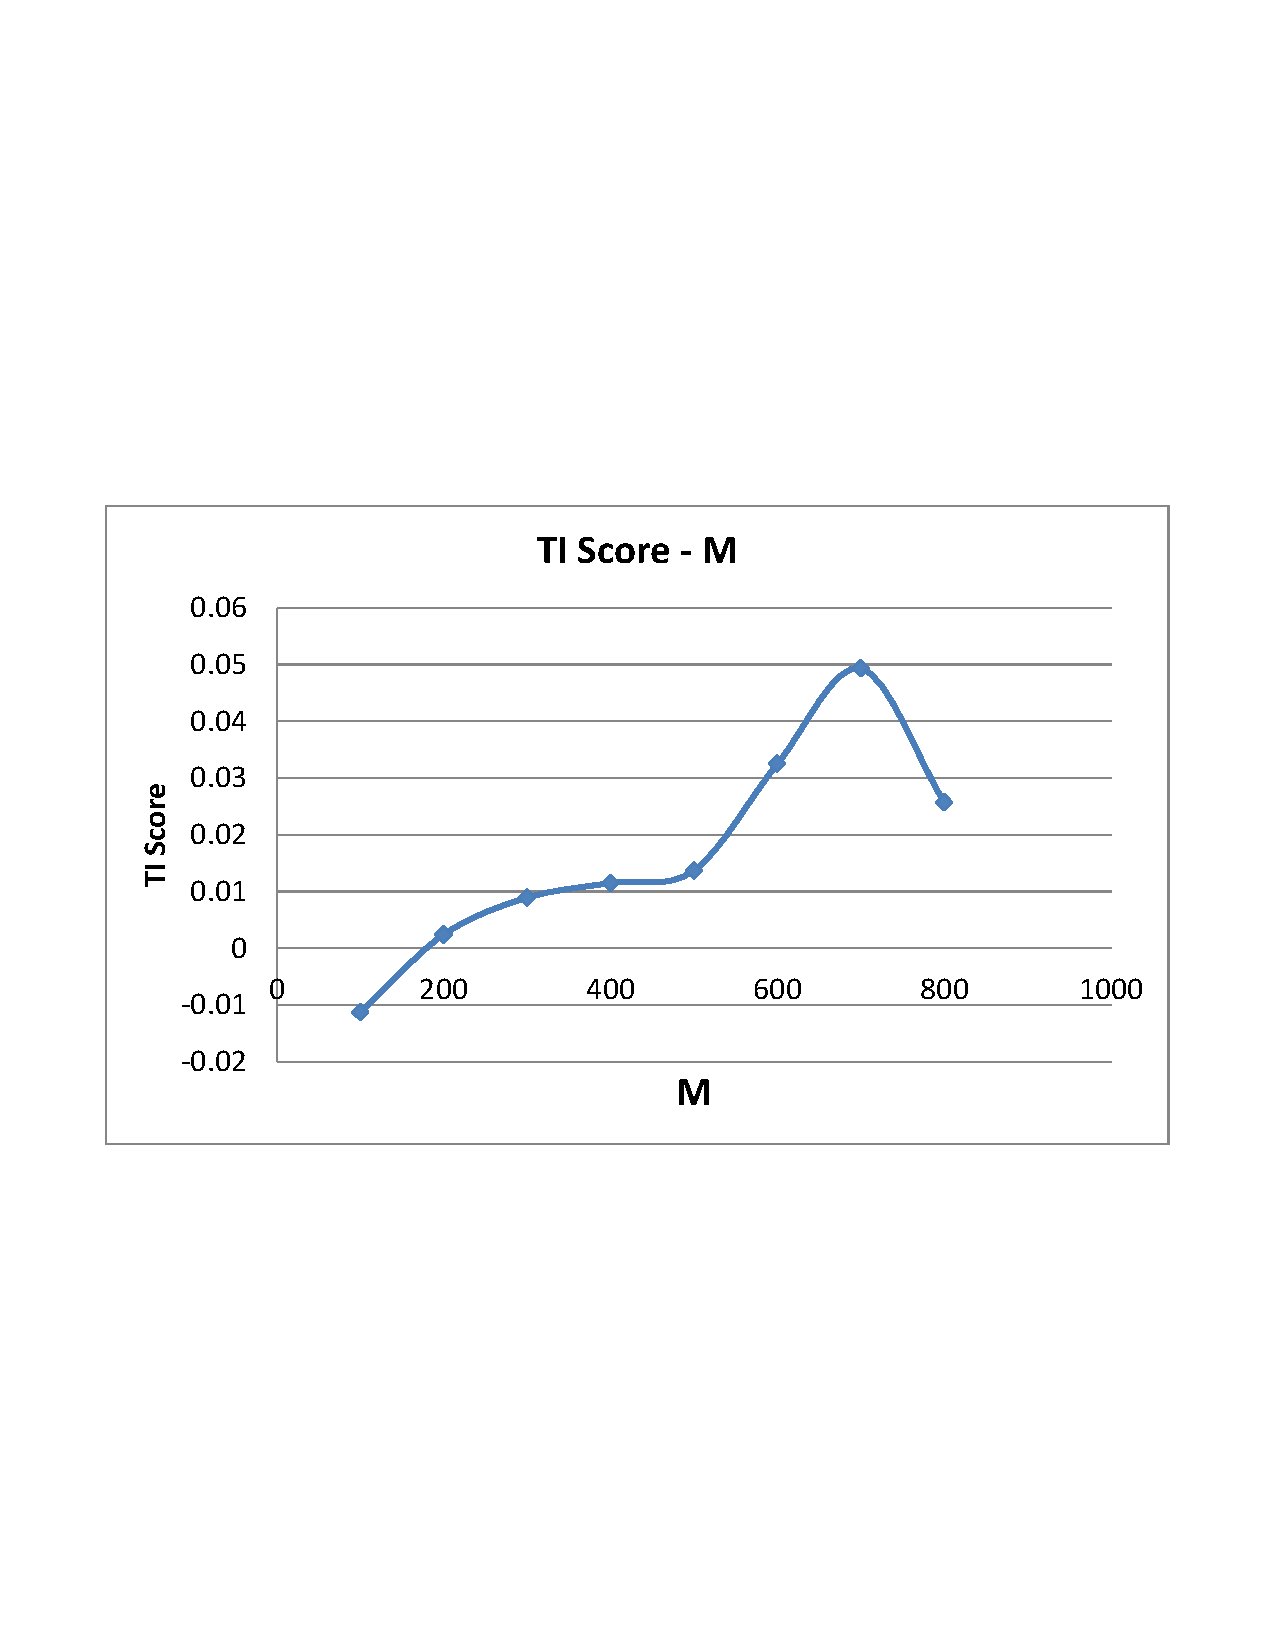
\includegraphics[width=0.5\linewidth]{figures/20news_M_TI_chart.pdf}
\caption{TI Score for word count thresholds $M$ on \textsc{20 news} group dataset.}
\label{fig:anchor-select}
\end{figure}











  

Since this {\bf anchor }algorithm is very sensitive to the extracted anchor words,
we can consider better ways to extract the anchor word candidates
rather than document frequency, for example, tf-idf, etc.




\paragraph{Regularization and Evaluation}

For a given word count cut-off, we can examine the trend of our evaluation
measures for different values of $\lambda$ and number of topics $K$ on our
develop set (Figure~\ref{fig:select-lambda}).  
For larger number of topics ($K > 20$), $L_2$ regularization improves held-out prediction,
and Beta regularization improves coherence ({\bf TI}).
However, when $K=20$, neither of the two regularization are better than {\bf
  anchor}; we hypothesize this is because there is sufficient data for each
topic to learn effective topics.

\begin{figure}[t!]
\centering
\subfigure{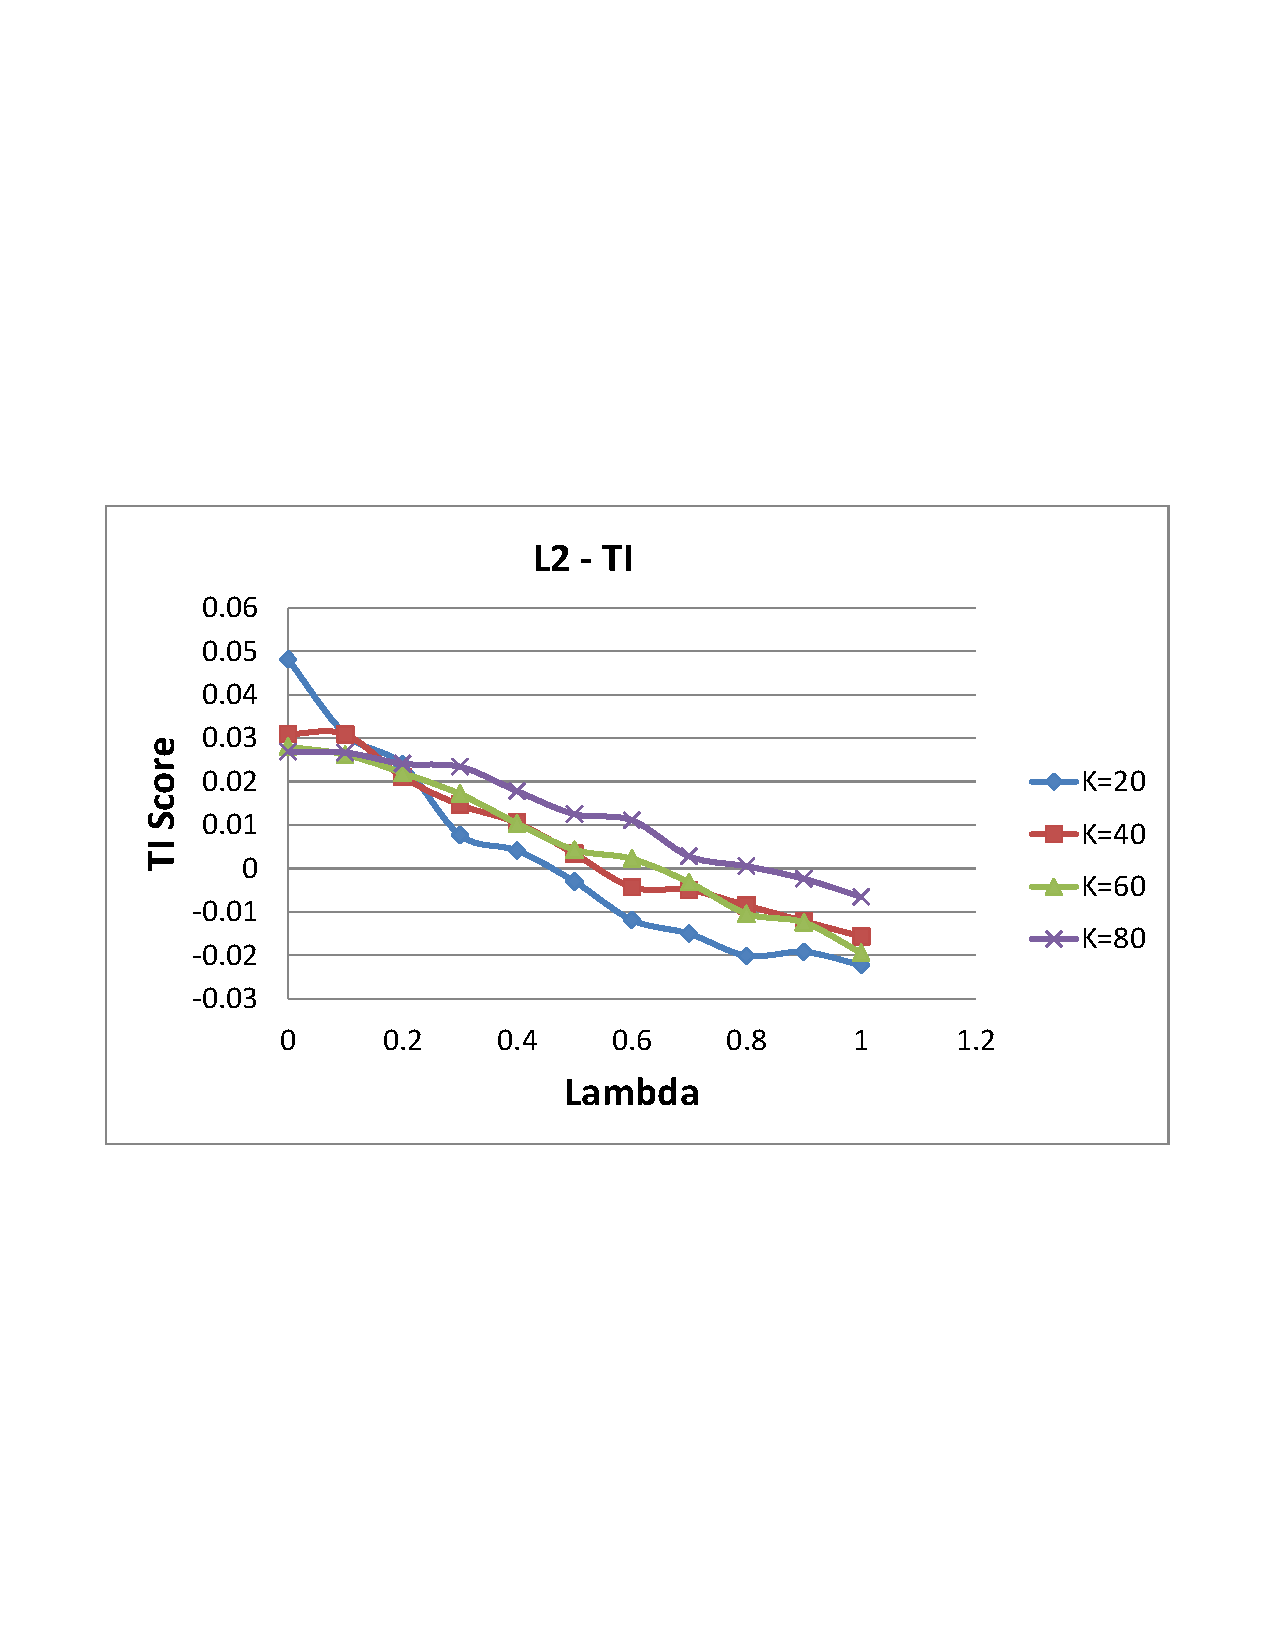
\includegraphics[width=0.48\linewidth]{figures/20news_700_TI.pdf}}
\hspace{0.1in}
\subfigure{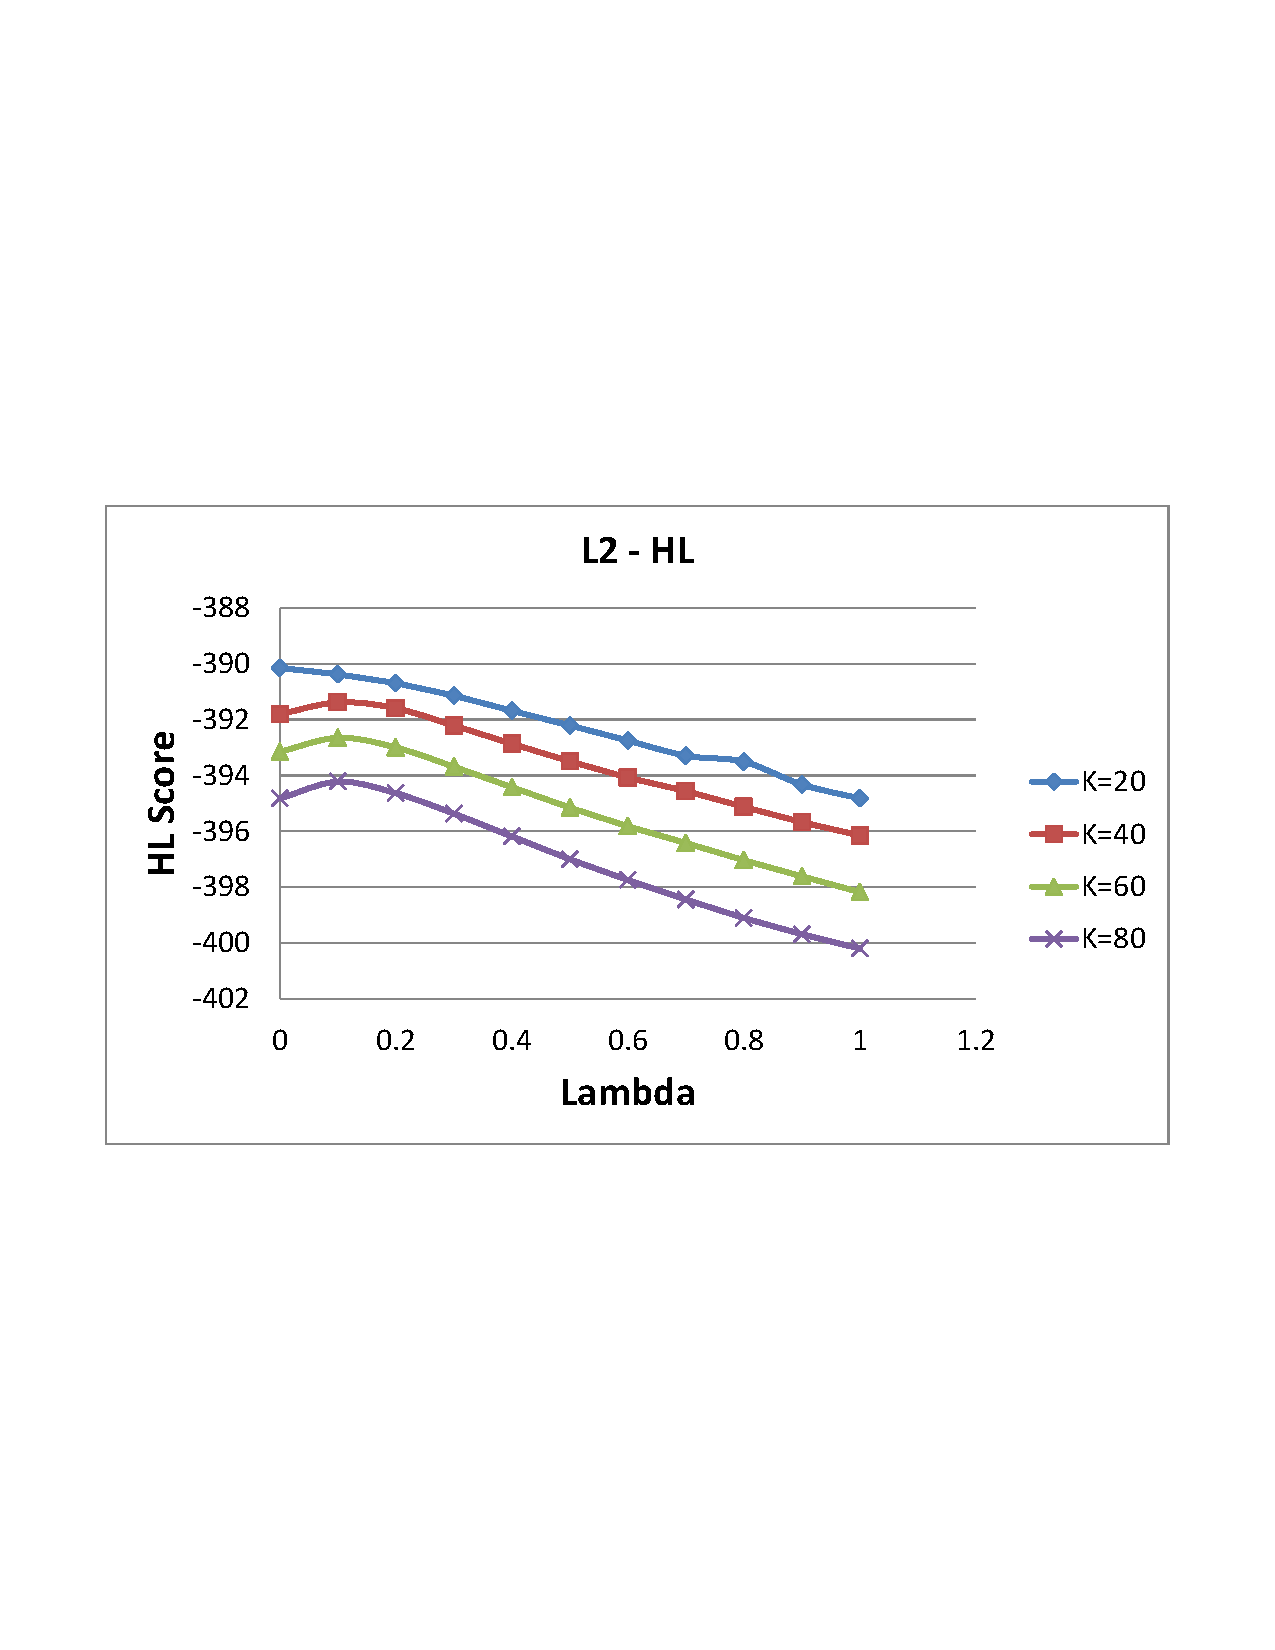
\includegraphics[width=0.48\linewidth]{figures/20news_700_Likelihood.pdf}}
\subfigure{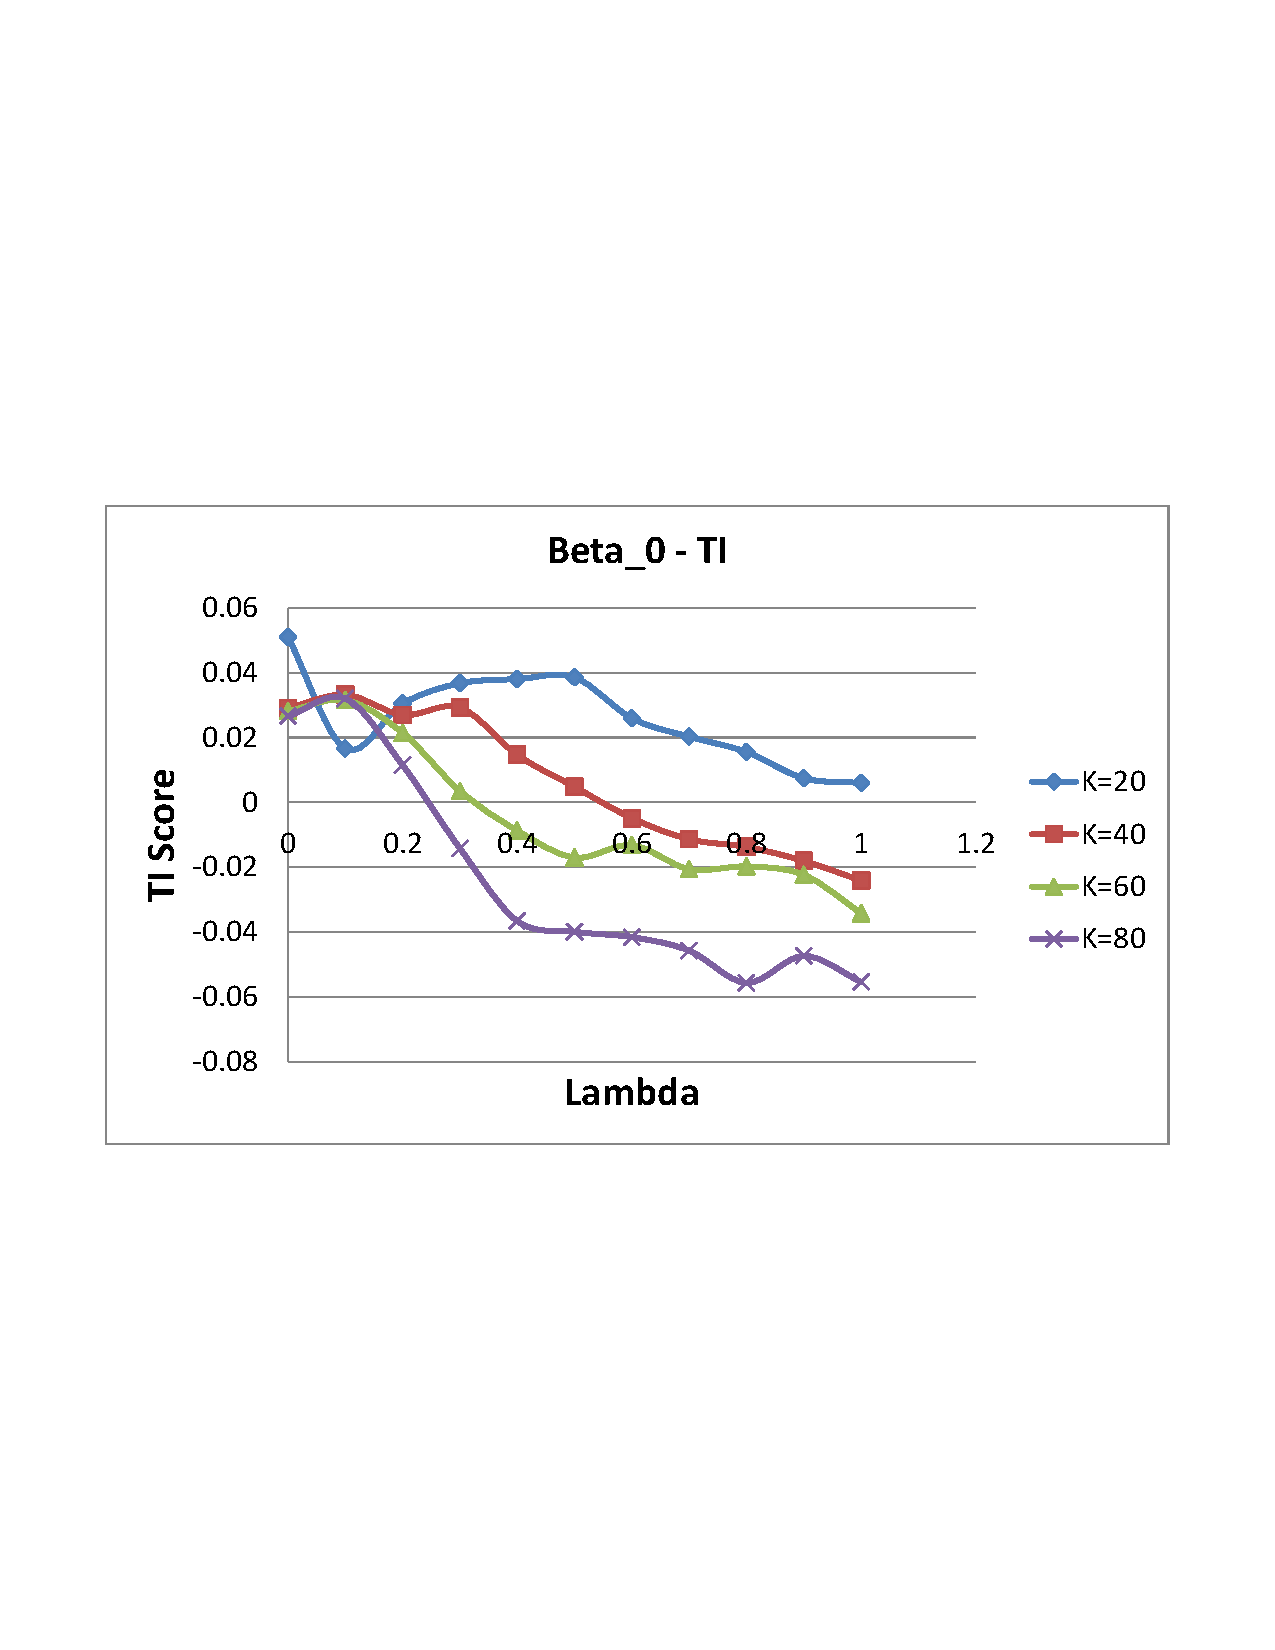
\includegraphics[width=0.48\linewidth]{figures/20news_700_TI_Beta.pdf}}
\hspace{0.1in}
\subfigure{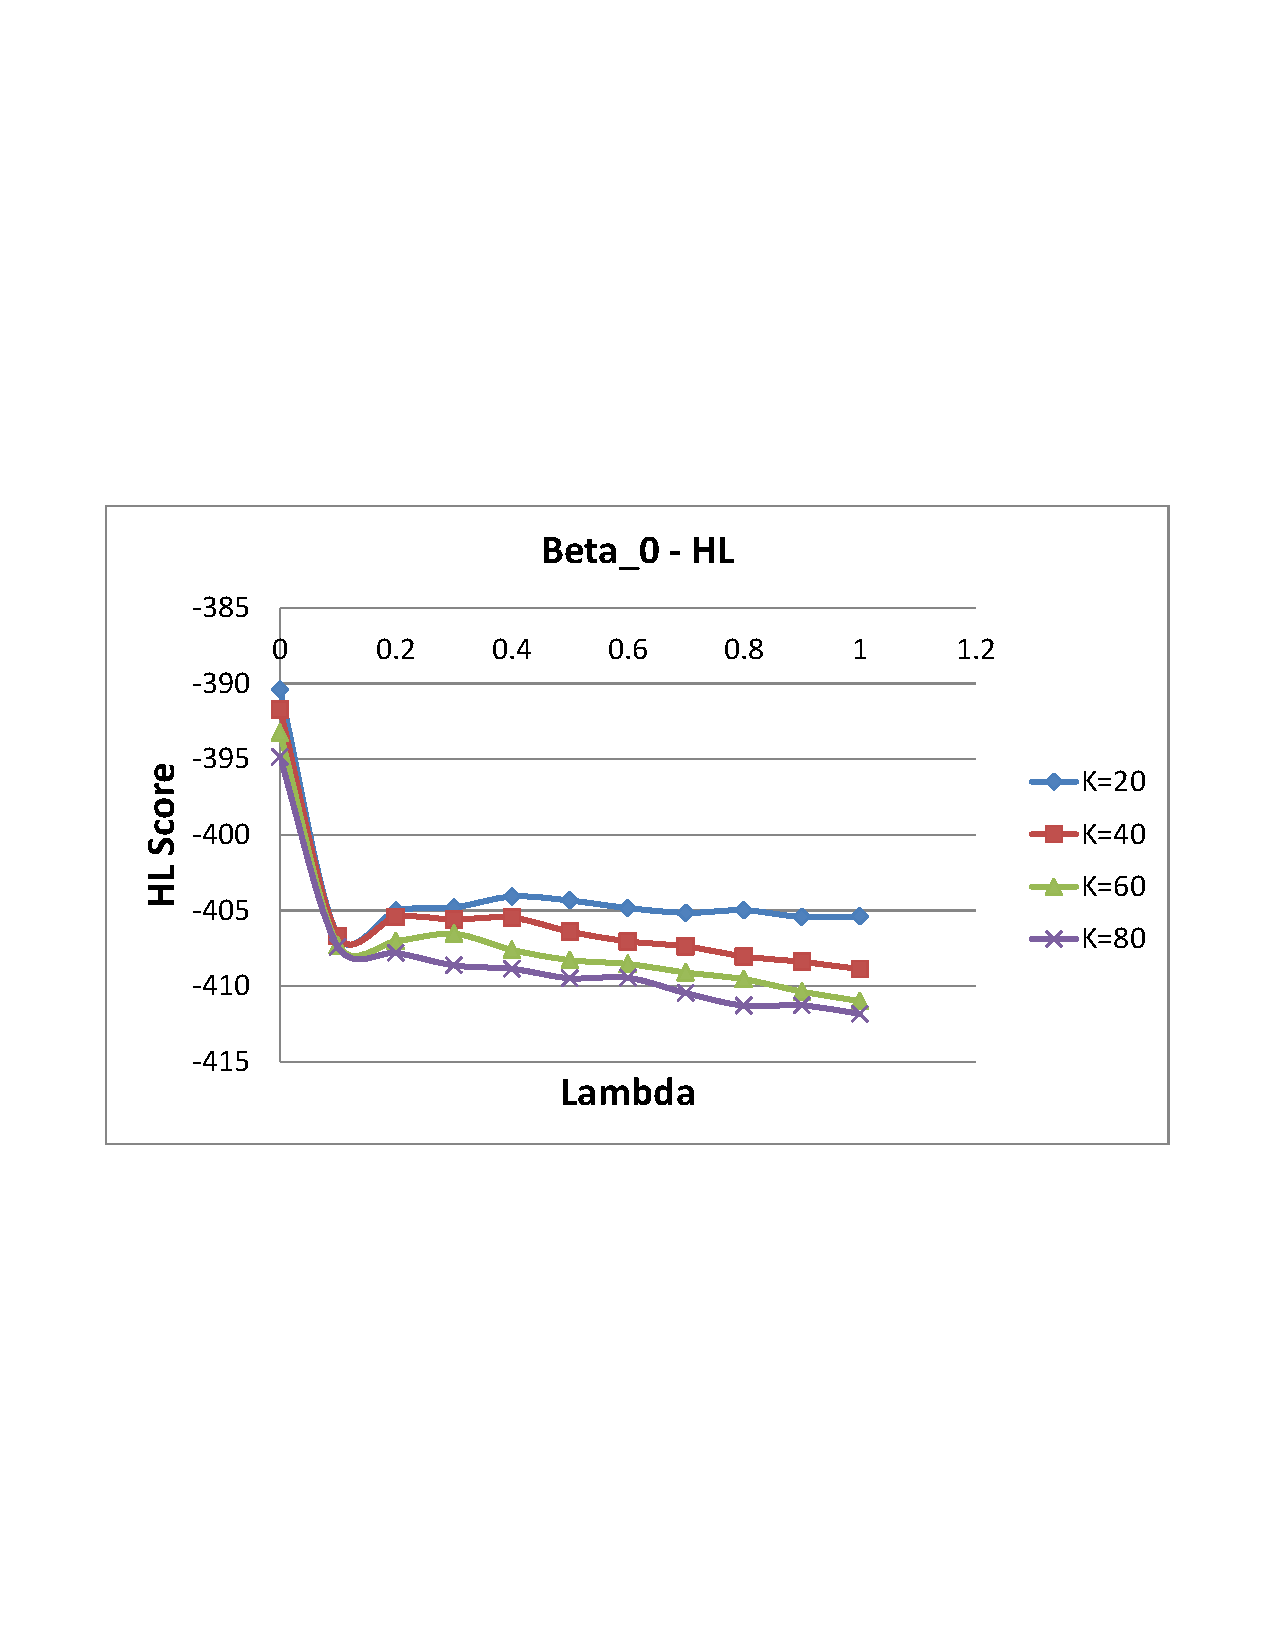
\includegraphics[width=0.48\linewidth]{figures/20news_700_Likelihood_Beta.pdf}}
\caption{TI Score and held-out likelihood score for $L_2$ regularization on 20news dataset, M = 700.}
\label{fig:select-lambda}
\end{figure}

\begin{comment}
Figure~\ref{fig:select-lambda} also shows that Beta regularization performs
very differently from the $L_2$ regularization. It may because that the $\hat C$ matrix
in Beta regularization was initialized with a Dirichlet distribution with parameter $\alpha$.
In addition, optimization
procedure for Beta regularization also suffers from premature convergence due
to the factor $\frac{1}{C_i}$  in the gradient.
\end{comment}


Given the parameters selected on development data, we apply these parameters to
test data (Table~\ref{tab:results}).  These obtained comparable results;
word-topic profiles are available in the Appendix~\ref{appendix:K40-LAMBDA0} and \ref{appendix:K40-LAMBDA0P1}.















































\section{Conclusion}

This paper introduces two different regularizations to spectral learning methods of topic
modeling, and evaluates the resulting topics using coherence and held-out
likelihood.  While the regularization did not show much effect when the topic
number is small, when the topic number became larger, $L_2$ improves heldout
likelihood score, and Beta regularization improves coherence.

We are investigating other regularizations such as $L_1$ regularization, using adaptive
settings of $\lambda$, and initializing the regularized models with the results
of unconstrained inference.


\begin{table}[t]
   \begin{center}
   \begin{footnotesize}
       \begin{tabular}{|c|cccc||cccc|} \hline
       	  & \multicolumn{4}{c||}{$\uparrow${\bf TI}} & \multicolumn{4}{c|}{$\uparrow${\bf HL}}\\ \hline
           &K=20 &K=40 &K=60 &K=80 &K=20 &K=40 &K=60 &K=80\\ \hline
          {\bf anchor} &{\bf 0.0499} &0.0314 &0.0277 &0.0255    &{\bf -407.4} &-408.8 &-410.5 &-411.9  \\
          {\bf anchor-$L_2$} &0.0318 &0.0273 &0.0255 &0.0256    &-407.5 &{\bf -408.0} &{\bf -409.8} &{\bf -411.3} \\
          {\bf anchor-beta} &0.0152 &{\bf 0.0326} &{\bf 0.0322} &{\bf 0.0321}   &-424.4 &-424.6 &-425.0 &-425.2\\
          \hline
       \end{tabular}
       \caption{Apply the selected parameters on the test data of \textsc{20 news}. {\bf anchor-beta} obtained
       better results on {\bf TI} score, while {\bf anchor-$L_2$} got slightly better results on $\bf HL$ score.
       }
       \label{tab:results}
   \end{footnotesize}
   \end{center}
\end{table}







\bibliographystyle{../style/nips}
\footnotesize
\bibliography{../bib/journal-abbrv,../bib/thang,../bib/jbg,../bib/ynhu}

\newpage
\section{Appendix}


\subsection{20news topics, K = 20, $\lambda=0$, $\lambda=0.1$, M = 100}
\label{appendix:K20-M100}

\begin{table}[h]
   \begin{center}
  \begin{tabular}{|c|c|l|} \hline
           Topic & Anchor word & Top 10 words \\ \hline
   Topic	1	&	max & max brain cheer clipper ticket pgp electrical andy traffic att	\\ \hline
Topic	2	&	van & van write win article doe team andrew april year email	\\ \hline
Topic	3	&	frequently & article write don doe make time people good system question	\\ \hline
Topic	4	&	debate & write article people make don doe key government time point	\\ \hline
Topic	5	&	stats & player write team game article stats year good play don	\\ \hline
Topic	6	&	danger & write article don people make system doe government problem good	\\ \hline
Topic	7	&	ignorance & write article don people god doe make post ignorance time	\\ \hline
Topic	8	&	wings & game team write wings article win red play hockey year	\\ \hline
Topic	9	&	mailing & email write list article doe address mailing internet mail people	\\ \hline
Topic	10	&	eternal & god write article don jesus people christian make time bible	\\ \hline
Topic	11	&	touch & write article don good make car time doe problem people	\\ \hline
Topic	12	&	letters & write article don email doe case make people good letters	\\ \hline
Topic	13	&	vga & drive card email doe windows monitor write sale system offer	\\ \hline
Topic	14	&	geb & write article don people gordon banks geb make good doe	\\ \hline
Topic	15	&	default & window write file problem article windows doe system make set	\\ \hline
Topic	16	&	armenia & armenian write people turkish article armenia war government israel jew	\\ \hline
Topic	17	&	compile & program write file email doe call windows problem don run	\\ \hline
Topic	18	&	update & windows file write driver system doe version email update problem	\\ \hline
Topic	19	&	period & write article period power play don game make good year	\\ \hline
Topic	20	&	plenty & write article don make people good doe car time work	\\ \hline

          \end{tabular}

       \label{tab:M100 topics}
   \end{center}
\vspace{-10pt}
\end{table}

\subsection{20news topics, K = 20, $\lambda=0$, $\lambda=0.1$, M = 700}
\label{appendix:K20-M700}

\begin{table}[h]
   \begin{center}
  \begin{tabular}{|c|c|l|} \hline
           Topic & Anchor word & Top 10 words \\ \hline
Topic	1	&	drive & drive disk hard scsi controller card problem floppy ide mac	\\ \hline
Topic	2	&	god & god jesus christian people bible faith church life christ belief	\\ \hline
Topic	3	&	game & game team player play win fan hockey season run baseball	\\ \hline
Topic	4	&	file & file windows ftp driver dos version site image directory problem	\\ \hline
Topic	5	&	article & article don people make time back good work isn doe	\\ \hline
Topic	6	&	list & list mailing address add people send post book marc interest	\\ \hline
Topic	7	&	program & program window call doe advance problem application run windows give	\\ \hline
Topic	8	&	power & power car play period good supply make ground light battery	\\ \hline
Topic	9	&	government & government people key state law make israel gun israeli encryption	\\ \hline
Topic	10	&	part & part max doe end air make cut western call include	\\ \hline
Topic	11	&	support & support doe driver card version mode video system information work	\\ \hline
Topic	12	&	group & group post don question posting people read time newsgroup create	\\ \hline
Topic	13	&	line & line problem window display set doe place point subject find	\\ \hline
Topic	14	&	computer & computer system phone university problem doe science means work windows	\\ \hline
Topic	15	&	year & year team good years player time win car make play	\\ \hline
Topic	16	&	buy & buy car price good bike doe don sell make cheap	\\ \hline
Topic	17	&	write & write don make people time good doe post back thing	\\ \hline
Topic	18	&	number & number don key call phone doe question order chip company	\\ \hline
Topic	19	&	john & john move internet receive doe black full jewish posting include	\\ \hline
Topic	20	&	email & email sale offer send address fax interest advance internet mail	\\ \hline


          \end{tabular}

       \label{tab:M700 topics}
   \end{center}
\vspace{-10pt}
\end{table}

\newpage


\subsection{20news topics, M = 700, K = 40, $\lambda=0$}
\label{appendix:K40-LAMBDA0}

\begin{table}[h]
   \begin{center}
  \begin{tabular}{|c|c|l|} \hline
           Topic & Anchor word & Top 10 words \\ \hline
Topic	1	&	drive & drive disk hard scsi controller card floppy ide mac problem	\\ \hline
Topic	2	&	god & god jesus christian people bible church christ life belief faith	\\ \hline
Topic	3	&	game & game team player play win fan hockey season run baseball	\\ \hline
Topic	4	&	file & file windows ftp driver dos version site image directory doe	\\ \hline
Topic	5	&	list & list mailing address add people doe marc send user mike	\\ \hline
Topic	6	&	article & article don people make bob back mark didn steve gordon	\\ \hline
Topic	7	&	program & program window advance doe windows run application display object user	\\ \hline
Topic	8	&	power & power car play period supply ground battery light high current	\\ \hline
Topic	9	&	part & part max doe end air cut make western individual pay	\\ \hline
Topic	10	&	support & support doe driver card version mode video cards graphics software	\\ \hline
Topic	11	&	government & government people key encryption law armenian public clipper make system	\\ \hline
Topic	12	&	line & line doe display subject place area screen find easy note	\\ \hline
Topic	13	&	group & group don question create discussion newsgroup posting wrong tom news	\\ \hline
Topic	14	&	computer & computer system phone means windows software problem mac quote screen	\\ \hline
Topic	15	&	write & write don make people good doe didn lot doesn opinion	\\ \hline
Topic	16	&	year & year team player years good win play car make big	\\ \hline
Topic	17	&	buy & buy car price good bike doe cheap sell card dealer	\\ \hline
Topic	18	&	email & email send address fax advance reply offer mail sale internet	\\ \hline
Topic	19	&	john & john move receive doe internet full jewish posting black tom	\\ \hline
Topic	20	&	order & order point don find question place net mail long give	\\ \hline
Topic	21	&	times & times time good doe joe tire method advice place point	\\ \hline
Topic	22	&	david & david guy time care internet koresh back don great netcomcom	\\ \hline
Topic	23	&	put & put back don make man space people time bike face	\\ \hline
Topic	24	&	number & number phone don key company question numbers chip answer read	\\ \hline
Topic	25	&	bit & bit key data speed fast work bike time chip problem	\\ \hline
Topic	26	&	hear & hear doug happen eat found patient slot problem true mark	\\ \hline
Topic	27	&	claim & claim people evidence israel doe make fact objective truth israeli	\\ \hline
Topic	28	&	information & information doe interest book data appreciated info find point source	\\ \hline
Topic	29	&	change & change problem don system similar make work start things turn	\\ \hline
Topic	30	&	university & university internet fax research science institute usa phone view department	\\ \hline
Topic	31	&	include & include sale offer condition price sell cover original good shipping	\\ \hline
Topic	32	&	real & real don test time posting people close work true doe	\\ \hline
Topic	33	&	kind & kind don max people doe lot dan soul age send	\\ \hline
Topic	34	&	post & post won posting faq read response doe message question final	\\ \hline
Topic	35	&	isn & isn henry keith andy clipper don work assume doe people	\\ \hline
Topic	36	&	bad & bad good don make time people problem experience things comment	\\ \hline
Topic	37	&	show & show men world child people faith time found study james	\\ \hline
Topic	38	&	set & set window problem work source command colors start doe color	\\ \hline
Topic	39	&	call & call don give make good case peter reply love friend	\\ \hline
Topic	40	&	state & state people bill law gun live country carry israel years	\\ \hline



          \end{tabular}

       \label{tab:M700_0 topics}
   \end{center}
\vspace{-10pt}
\end{table}

\newpage

\subsection{20news topics, M = 700, K = 40, $\lambda=0.1$, {\bf anchor-beta}}
\label{appendix:K40-LAMBDA0P1}

\begin{table}[h]
   \begin{center}
  \begin{tabular}{|c|c|l|} \hline
           Topic & Anchor word & Top 10 words \\ \hline

Topic	1	&	drive & drive card software hard data mac disk machine monitor speed	\\ \hline
Topic	2	&	god & god true reason life man christian person love exist assume	\\ \hline
Topic	3	&	file & file windows advance driver version found source works check memory	\\ \hline
Topic	4	&	game & game team play mike player home win fan guy season	\\ \hline
Topic	5	&	government & key government pay chip law today issue public gun kill	\\ \hline
Topic	6	&	list & list add white class complete texas cheer count mailing marc	\\ \hline
Topic	7	&	article & article dave bob brain gordon doctor fit banks andrew foot	\\ \hline
Topic	8	&	program & program window application simple manager function object algorithm values associate	\\ \hline
Topic	9	&	power & power light special supply ground period unit washington battery circuit	\\ \hline
Topic	10	&	part & part end max air cut mile individual begin parts ron	\\ \hline
Topic	11	&	group & group posting deal tom newsgroup folks specific reader personally curious	\\ \hline
Topic	12	&	support & support mode mouse cards release higher motif technical greg resolution	\\ \hline
Topic	13	&	computer & computer phone means quote pro ray ship electronic processor corp	\\ \hline
Topic	14	&	line & line signal draw noise wall distribution led newsgroups bottom drawing	\\ \hline
Topic	15	&	buy & buy price bike current cost cheap thinking engine ride worth	\\ \hline
Topic	16	&	write & write don make people good time system problem work question	\\ \hline
Topic	17	&	number & number doe prefer professional charles exact procedure equivalent telephone comparison	\\ \hline
Topic	18	&	year & year top city numbers early past smith san stay george	\\ \hline
Topic	19	&	bit & bit suggest stick clock doe turning operations random jump rate	\\ \hline
Topic	20	&	email & email internet send address info fax mail offer reply sell	\\ \hline
Topic	21	&	john & john move receive jewish letters weren doe black cross brain	\\ \hline
Topic	22	&	hear & hear food doug slot disease dog eat hours patient hall	\\ \hline
Topic	23	&	order & order tony equipment piece cross finger bell warning technique doe	\\ \hline
Topic	24	&	real & real test close vehicle treat planet doe art posting letters	\\ \hline
Topic	25	&	times & times advice page tire pain heavy enter doe central length	\\ \hline
Topic	26	&	change & change similar normal avoid hole oil review exact larger drink	\\ \hline
Topic	27	&	university & university research technology science view usa radio school major department	\\ \hline
Topic	28	&	david & david koresh stephen guy fly doe cambridge shoot stupid highly	\\ \hline
Topic	29	&	put & put pull moon putting keeping doe conditions potential shut wheel	\\ \hline
Topic	30	&	claim & claim evidence israel study taking objective frank water finally driving	\\ \hline
Topic	31	&	information & information appreciated reference project chips development medical services andor surface	\\ \hline
Topic	32	&	include & include cover imagine remote shape art doe originally open item	\\ \hline
Topic	33	&	kind & kind break dan trouble age park soul douglas eye guide	\\ \hline
Topic	34	&	post & post won response product thread description familiar doe writer topic	\\ \hline
Topic	35	&	set & set size event character colors reduce default background keyboard parent	\\ \hline
Topic	36	&	isn & isn henry andy listen flight fred remind wear baby doe	\\ \hline
Topic	37	&	long & long orbit quickly doe mix putting foot hole lock lab	\\ \hline
Topic	38	&	call & call peter entire paint frame style table doe solid att	\\ \hline
Topic	39	&	bad & bad comment pat riding damage cop truck sick handling finding	\\ \hline
Topic	40	&	show & show inside straight sex johnson pressure sexual male doe complain	\\ \hline




          \end{tabular}

       \label{tab:M700_0_1 topics}
   \end{center}
\vspace{-10pt}
\end{table}





\end{document}